% document class
\documentclass{scrartcl}

% encoding
\usepackage[T1]{fontenc}
\usepackage[utf8]{inputenc}%utf8

% language
\usepackage[ngerman]{babel}
\usepackage{scrhack} % nach \documentclass
\usepackage[aux]{rerunfilecheck}
\usepackage{polyglossia}
\setmainlanguage{german}

% math
\usepackage{amsmath}
\usepackage{amsfonts}
\usepackage{amssymb}
\usepackage{amstext}
\usepackage{isomath}
\usepackage{mathtools}

% physics
\usepackage{tensor}
\usepackage{slashed}
\usepackage{braket}
\usepackage[strict, separate-uncertainty, sticky-per]{siunitx}

% fonts
\usepackage{microtype}
\usepackage{fourier}
\usepackage{tgheros}
\usepackage{tgcursor}
\usepackage{tgpagella}

% tikz
\usepackage{tikz}

% margins
\usepackage[top=2.5cm]{geometry}

% variables
\newcommand{\thehandover}{Freitag, den 20.\,Oktober 2017 12:00 Uhr}
\newcommand{\thesheet}{1}
\newcommand{\thesemester}{WS 17/18}
\newcommand{\theprofessor}{Priv.-Doz.~U.~Löw}

% enumeration
\renewcommand{\labelenumi}{(\alph{enumi})} % alphabetic tasks
\renewcommand{\theenumi}{(\alph{enumi})} % alphabetic tasks
\usepackage{enumitem} % allows to continue lists with [resume]

% clickable links and '\url' command
\usepackage[hidelinks]{hyperref}

\usepackage{placeins}



\newcommand{\ua}[1]{_\symup{#1}}
\newcommand{\su}[1]{\symup{#1}}


\begin{document}


\begin{figure}[h]
  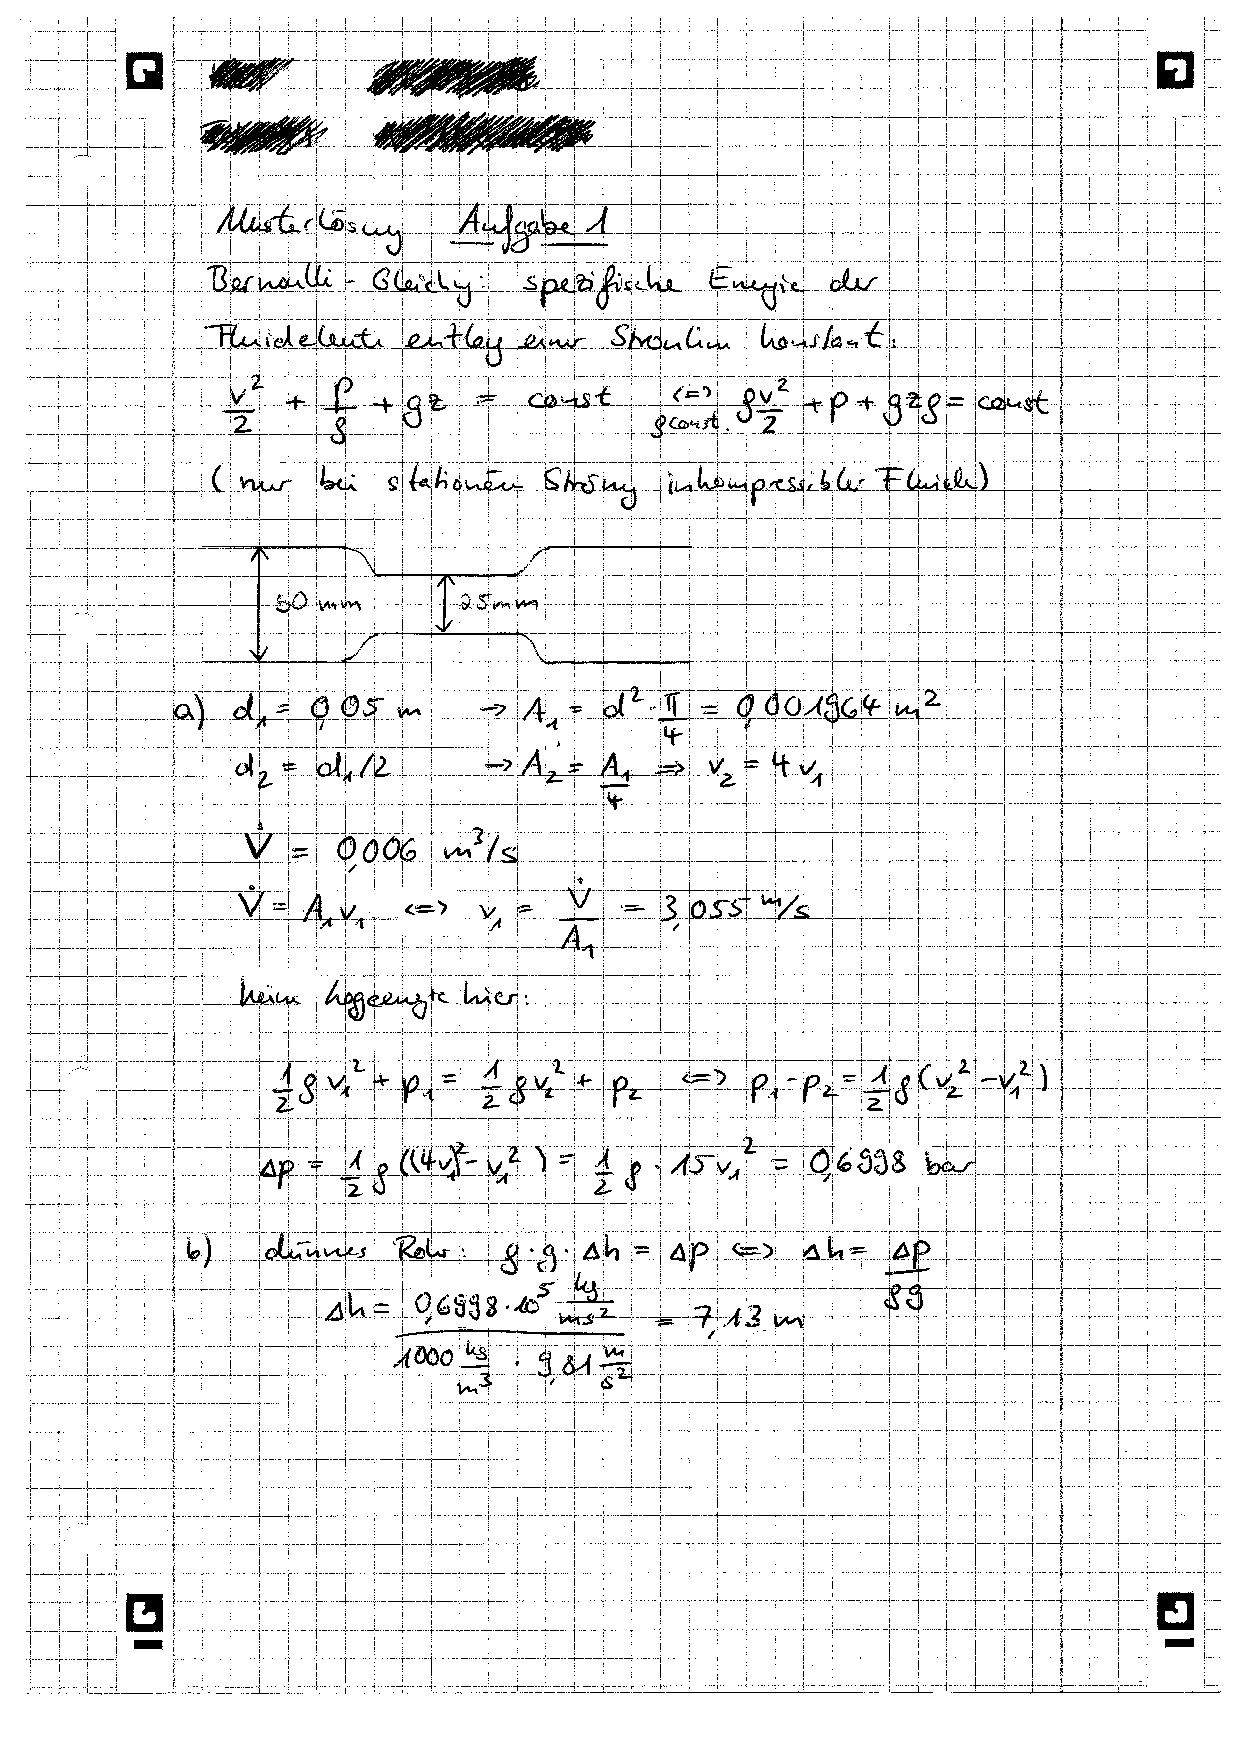
\includegraphics[width = \textwidth]{LoesungRohr.pdf}
\end{figure}

\textbf{Musterlösung: Navier-Stokes}

\begin{itemize}
  \item[a.)]
    \begin{align*}
      v_x =& v_y = 0\\
      v_z =& v(r)\\
      \Rightarrow \Delta V =& \frac{1}{r}\frac{\text{d}}{\text{d}r}
      \left(r\frac{\text{d}v}{\text{d}r}\right) = 0
    \end{align*}
  \item[b.)]
    \begin{align*}
      v(r = R_1) =& u\\
      v(r = R_2) =& 0
    \end{align*}
  \item[c.)]
    \begin{align*}
      \frac{\text{d}}{\text{d}r}
      \left(r\frac{\text{d}v}{\text{d}r}\right) = 0\\
      \frac{\text{d}v}{\text{d}r} = \frac{c_1}{r}\\
      v(r) = c_1\cdot \ln{r} + c_2\\
      \text{Jetzt in die Randedingungen einsetzen:}\\
      \\
      u = v(R_1) =& c_1 \cdot \ln{R_1} + c_2\\
      0 = v(R_2) =& c_1 \cdot \ln{R_2} + c_2\\
      \Rightarrow c_1 = \frac{u}{\ln{\frac{R_1}{R_2}}} &
      c_2 = -\frac{u\ln{R_2}}{\ln{\frac{R_1}{R_2}}}\\
      \text{Ergebnis:}\\
      v(r) =& u\cdot\frac{\ln{\frac{r}{R_2}}}{\ln{\frac{R_1}{R_2}}}
    \end{align*}
\end{itemize}

\begin{figure}
  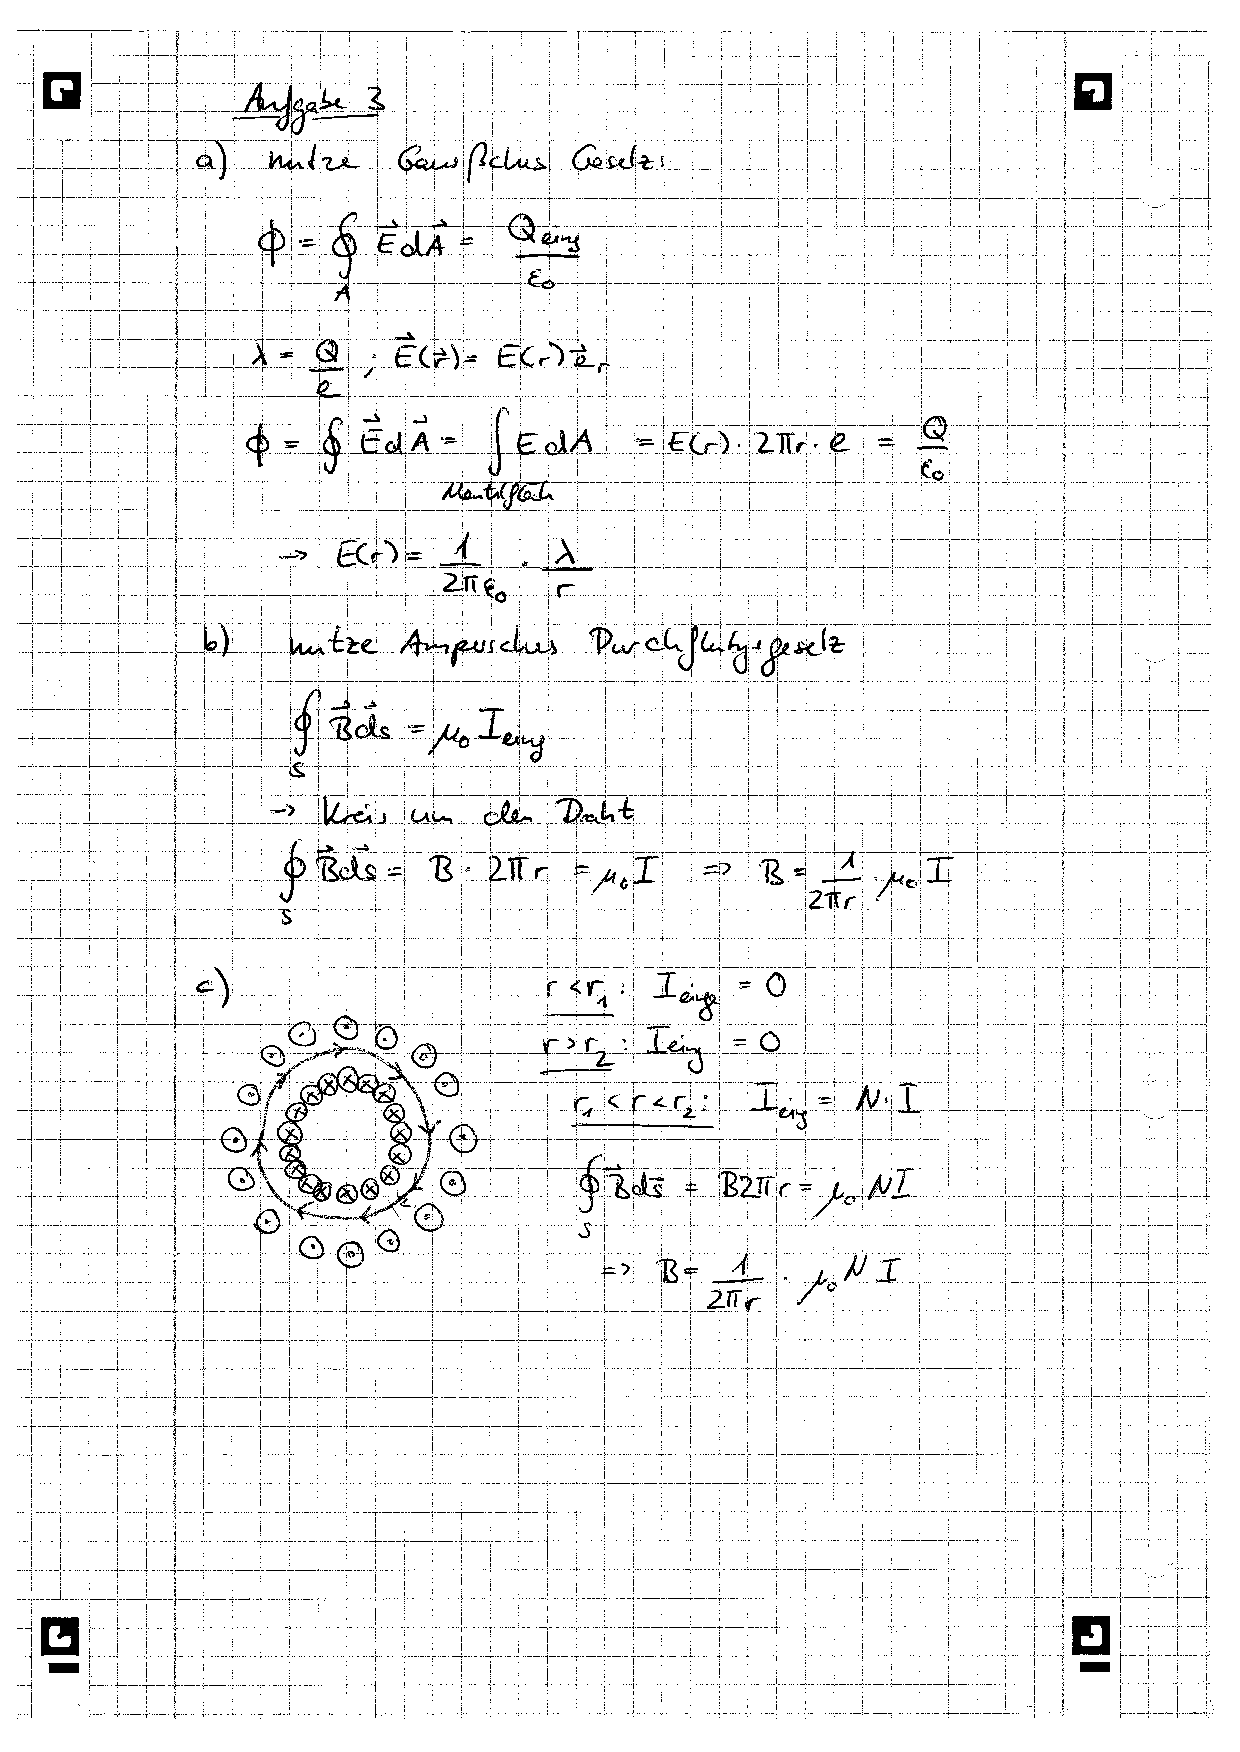
\includegraphics[width = \textwidth]{LoesungZusatz.pdf}
\end{figure}

\end{document}
